% !TeX encoding = UTF-8
\documentclass[aspectratio=169]{beamer}
\useoutertheme[progressbar=frametitle]{metropolis}
\useinnertheme{metropolis}
\definecolor{nabgray}{rgb}{0.6,0.59,0.61}
\usecolortheme[named=nabgray]{structure}
\usepackage{fontawesome5}
\usepackage{tikz}
\usepackage[utf8]{inputenc}
\usepackage[brazilian]{babel}
\usepackage{fontspec}
\setmonofont{JetBrains Mono}
\setmainfont{Helvetica Neue}
\setsansfont{Helvetica Neue}

\usepackage{smartdiagram}
\usepackage{qtree}
\usepackage{verbatim}
\usepackage{svg}
\usepackage{graphicx}
\usepackage{color}

\definecolor{lightgray}{rgb}{0.95, 0.95, 0.95}
\definecolor{darkgray}{rgb}{0.4, 0.4, 0.4}
%\definecolor{purple}{rgb}{0.65, 0.12, 0.82}
\definecolor{editorGray}{rgb}{0.95, 0.95, 0.95}
\definecolor{editorOcher}{rgb}{1, 0.5, 0} % #FF7F00 -> rgb(239, 169, 0)
\definecolor{editorGreen}{rgb}{0, 0.5, 0} % #007C00 -> rgb(0, 124, 0)
\definecolor{orange}{rgb}{1,0.45,0.13}
\definecolor{olive}{rgb}{0.17,0.59,0.20}
\definecolor{brown}{rgb}{0.69,0.31,0.31}
\definecolor{purple}{rgb}{0.38,0.18,0.81}
\definecolor{lightblue}{rgb}{0.1,0.57,0.7}
\definecolor{lightred}{rgb}{1,0.4,0.5}
\usepackage{upquote}
\usepackage{listings}
\lstset{language=java,
	basicstyle=\footnotesize\ttfamily,
	keywordstyle=\footnotesize\color{blue}\ttfamily,
	escapeinside={<@}{@>}
}

\usebackgroundtemplate%
{%
	
\includegraphics[width=\paperwidth]{Images/Contenido}%
}

\title{OpenTelemetry: A língua franca da observabilidade}
\subtitle{Você não pode melhorar o que não pode medir}
\author{Nabenik}
\date{\today}

\begin{document}
	
	{
		\usebackgroundtemplate{
\includegraphics[width=\paperwidth]{Images/portada}}
		\begin{frame}
			\maketitle
		\end{frame}
	}
	
	\begin{frame}{Observabilidade e monitoramento}
		
		\begin{columns}
			
			\begin{column}{0.5\textwidth}
				Sistema de TI {\Huge \faServer}
				\begin{itemize}
					\item Aplicações
					\item Serviços de terceiros
					\item Processos intermédios
					\item Hosts
				\end{itemize}
			\end{column}
			
			\begin{column}{0.5\textwidth}
				Fontes de informação {\Huge	 \faBinoculars}
				\begin{itemize}
					\item Eventos
					\item Logs
					\item Métricas
					\item Traces
				\end{itemize}
			\end{column}
		\end{columns}
		Teoria: Coletamos dados, processamos para identificar KPIs (golden signals) e criamos alarmes 
	\end{frame}


\begin{frame}{Observabilidade e monitoramento}
	
			Sistema de TI {\Huge \faServer}
			\begin{itemize}
				\item Aplicações: Binario (Go, GraalVM Native), minified (JS), jar, war (Java), K8s (containers), FaaS
				\item Serviços de terceiros (PaaS especializados)
				\item Processos intermédios (Banco de dados, message queue)
				\item Hosts (LSB, Alpine, openrc, Windows, etc.)
				\item ElasticSearch, Grafana, Datadog, New Relic, Cloudwatch, etc.
			\end{itemize}
	
\end{frame}

\begin{frame}{Observabilidade e monitoramento}
	
	Fontes de informação {\Huge	 \faBinoculars}
	\begin{itemize}
		\item Logs: Arquivos (/var/log), Systemd, FluentD
		\item Metrics: Hosts, JMX, Prometheus endpoints (Spring Actuator, Microprofile Metrics) 
		\item Traces: Jaeger, Zipkin
	\end{itemize}
	
\end{frame}

\begin{frame}{Observabilidade e monitoramento}
		Precisamos dados de \textbf{fontes e formatos diversos}, os quais podem ser \textbf{enviados ou coletados} para ser analisados em \textbf{plataformas de observabilidade} com diversas capacidades e riscos -e.g. Vendor lock in, tecnologias muito especificas, incompatibilidade entre versões- 
	
	\begin{alertblock}{Precisamos ...}
	data pipelines de observabilidade baseados numa \textbf{especificação} padrão
	\end{alertblock}
	
\end{frame}
	
%	{
%		\usebackgroundtemplate{
\includegraphics[width=\paperwidth]{Images/separador}}
%		\setbeamercolor{normal text}{fg=white}
%		\setbeamercolor{frametitle}{fg=red}
%		\usebeamercolor[fg]{normal text}
%		\section{Fontes de dados}
%	}
%	
%	\begin{frame}{Logs}
%		
%		\begin{block}{Definição}
%			Registro histórico de processos, eventos e mensagens com dados adicionais como timestamps e contexto
%		\end{block}	
%		Modo clássico
%		\begin{itemize}
%			\item Arquivos no sistema
%			\item Systemd
%			\item FluentD
%		\end{itemize}	
%	\end{frame}
%	
%	\begin{frame}
%		\begin{figure}
%			\centering
%			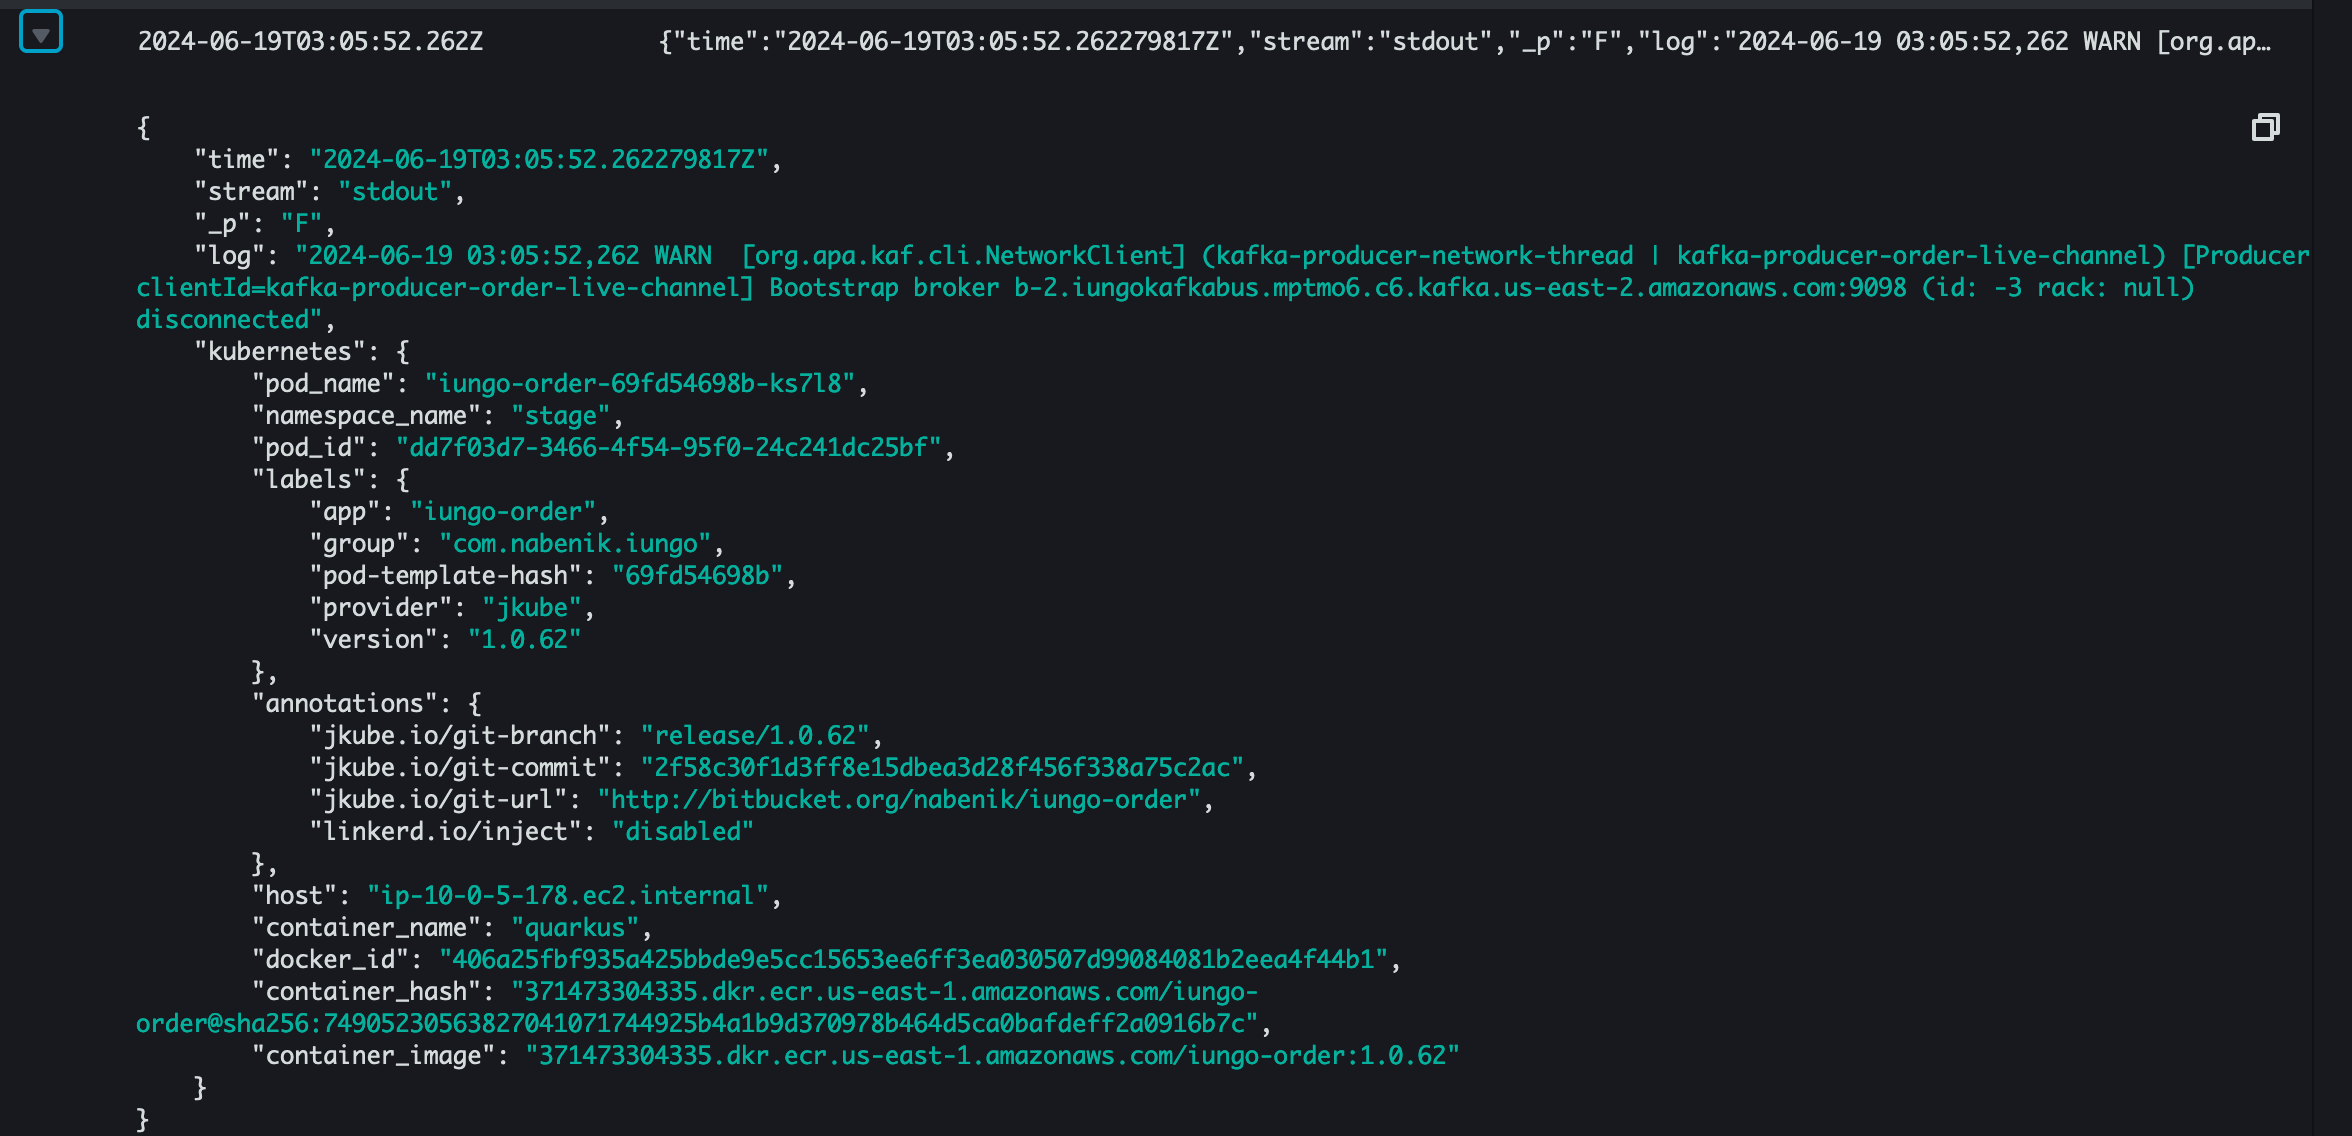
\includegraphics[width=0.8\linewidth]{Images/logs-sample}
%			\label{fig:logs-sample}
%		\end{figure}
%	\end{frame}
%	
%	\begin{frame}{Métricas}
%		
%		\begin{block}{Definição}
%			Valores numéricos sobre o desempenho das aplicações -e.g. Desempenho da rede, tamanho do heap-
%		\end{block}	
%		Formatos
%		\begin{itemize}
%			\item Gauge (instantâneos)
%			\item Delta (diferença entre dois pontos)
%			\item Acumulativas (mudanças ao longo do tempo)
%		\end{itemize}
%		
%		Modo clássico
%		\begin{itemize}
%			\item Sistema operacional
%			\item JMX
%			\item Endpoint HTTP (/actuator/metrics) - ServiceMonitor
%		\end{itemize}	
%	\end{frame}
%	
%	\begin{frame}
%		\begin{figure}
%			\centering
%			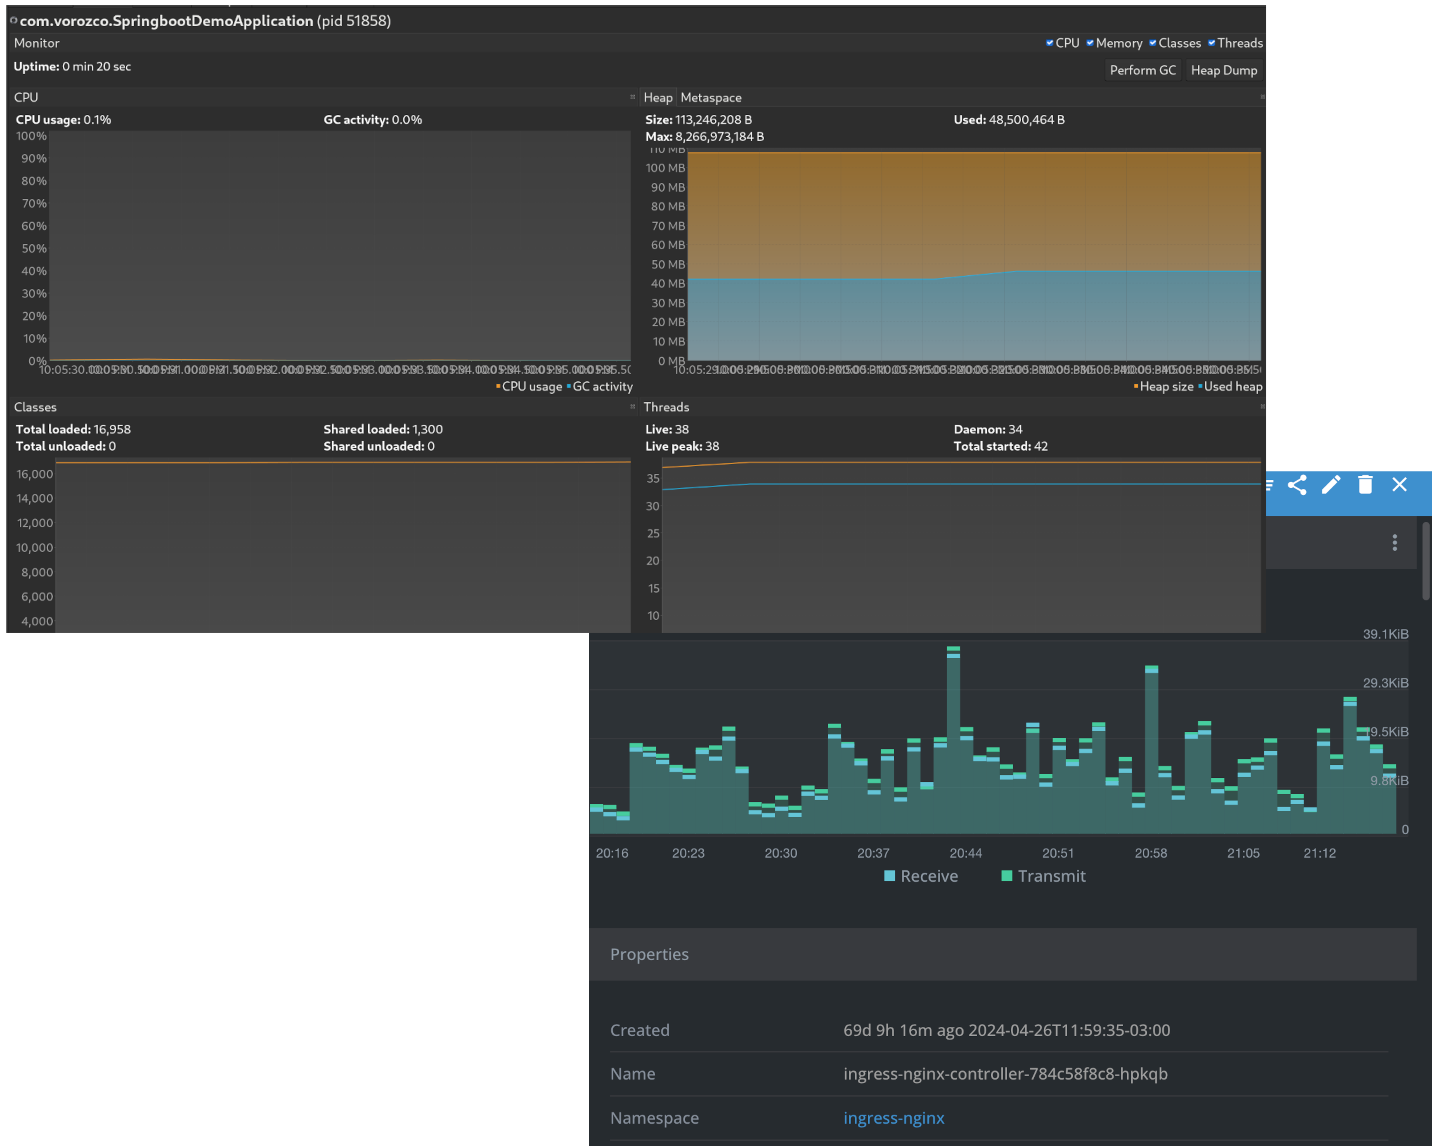
\includegraphics[width=0.7\linewidth]{Images/metrics-sample}
%			\label{fig:metrics-sample}
%		\end{figure}
%	\end{frame}
%	
%	\begin{frame}{Trace}
%		
%		\begin{block}{Definição}
%			Caminho completo de uma operação dentro de uma série de sistemas inter-relacionados. Cada participante cria spans que juntos formam os traces
%		\end{block}	
%		Modo clássico
%		\begin{itemize}
%			\item Protocolos push proprietários -e.g. Jaeger, Zipkin-
%		\end{itemize}	
%	\end{frame}
%	
%	\begin{frame}
%		\begin{figure}
%			\centering
%			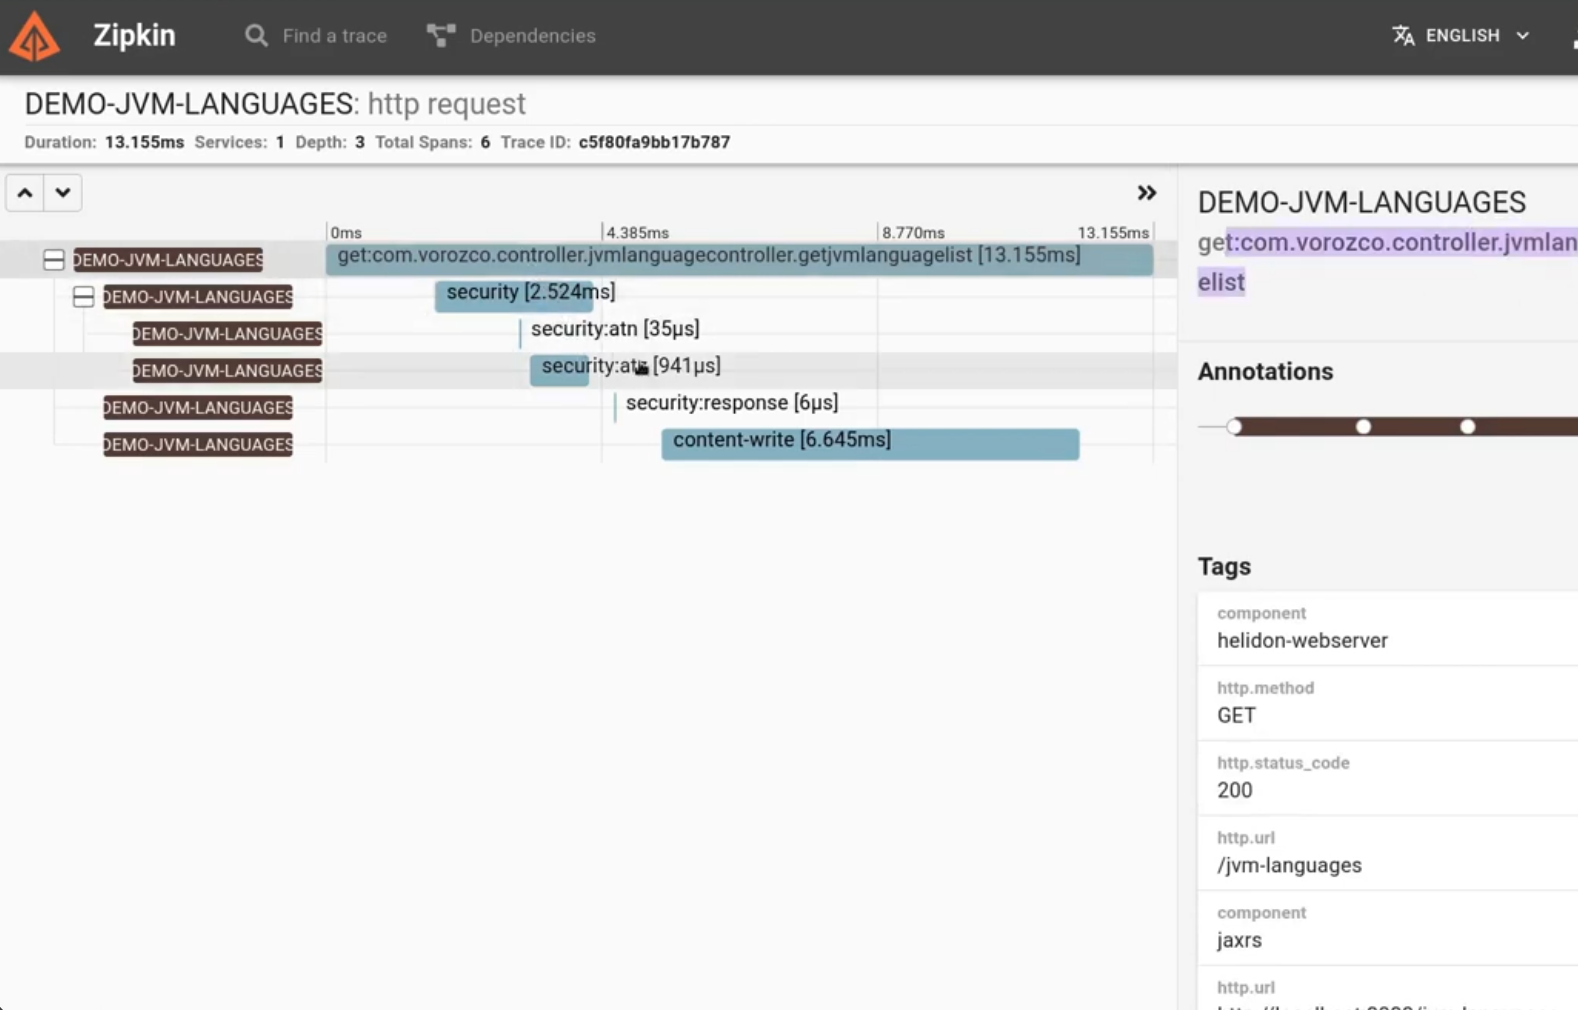
\includegraphics[width=0.7\linewidth]{Images/trace-sample}
%			\label{fig:trace-sample}
%		\end{figure}
%	\end{frame}
%	
	{
		\usebackgroundtemplate{
\includegraphics[width=\paperwidth]{Images/separador}}
		\setbeamercolor{normal text}{fg=white}
		\setbeamercolor{frametitle}{fg=red}
		\usebeamercolor[fg]{normal text}
		\section{OpenTelemetry}
	}
	
	
	\begin{frame}
		\begin{figure}
			\centering
			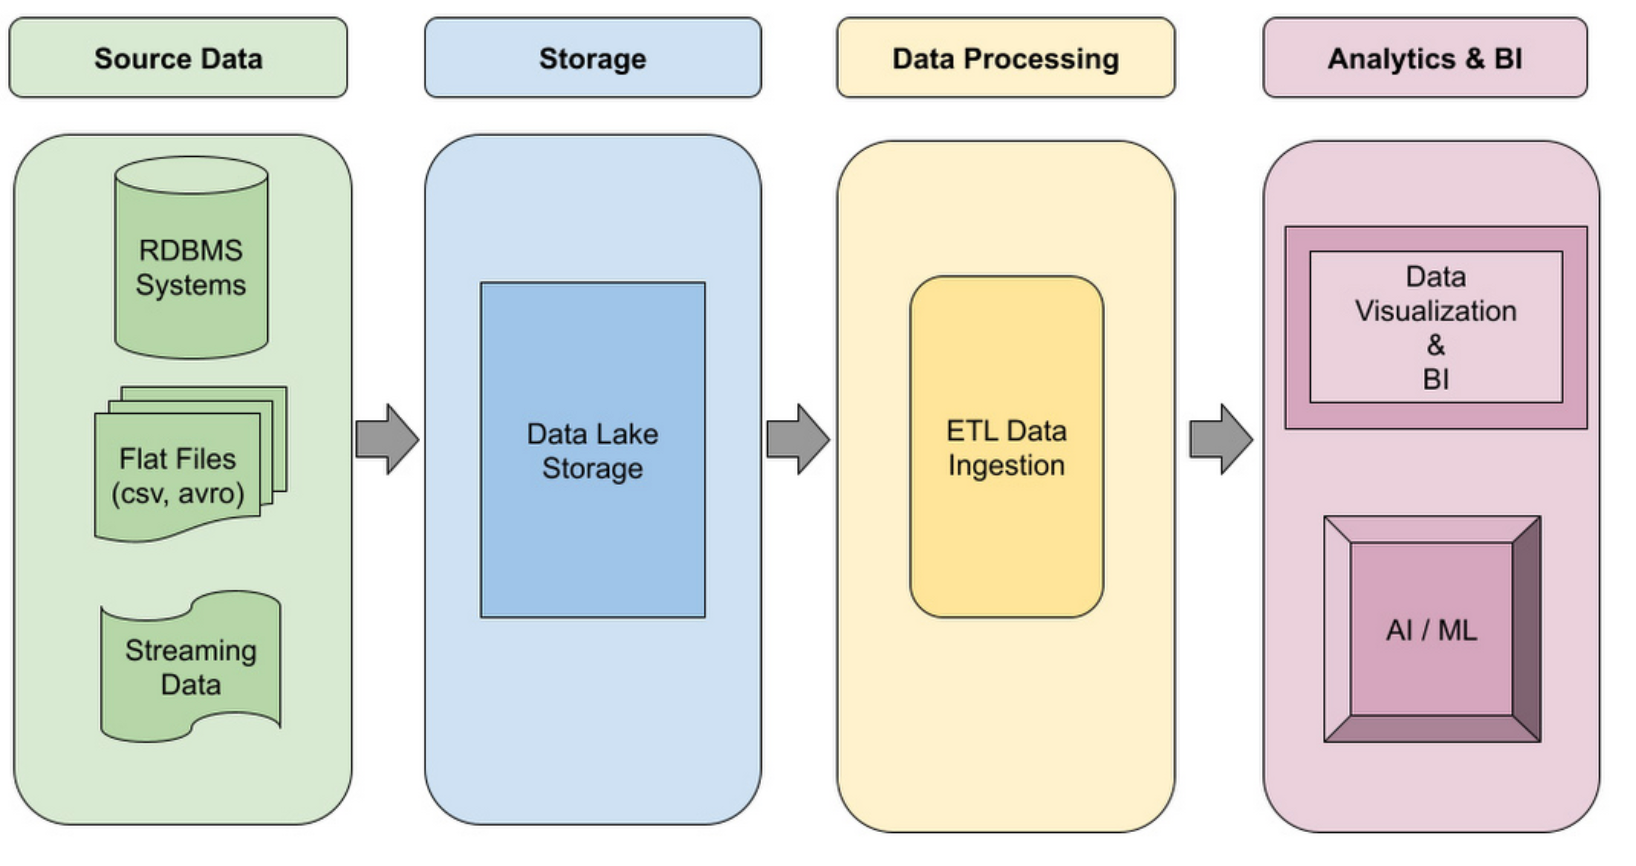
\includegraphics[width=0.8\linewidth]{Images/datalake}
			\label{fig:datalake}
			\caption{Data pipeline}
		\end{figure}
	\end{frame}
	
	
	\begin{frame}
		
		\begin{columns}
			\begin{column}{0.75\textwidth}
				\begin{figure}
					\centering
					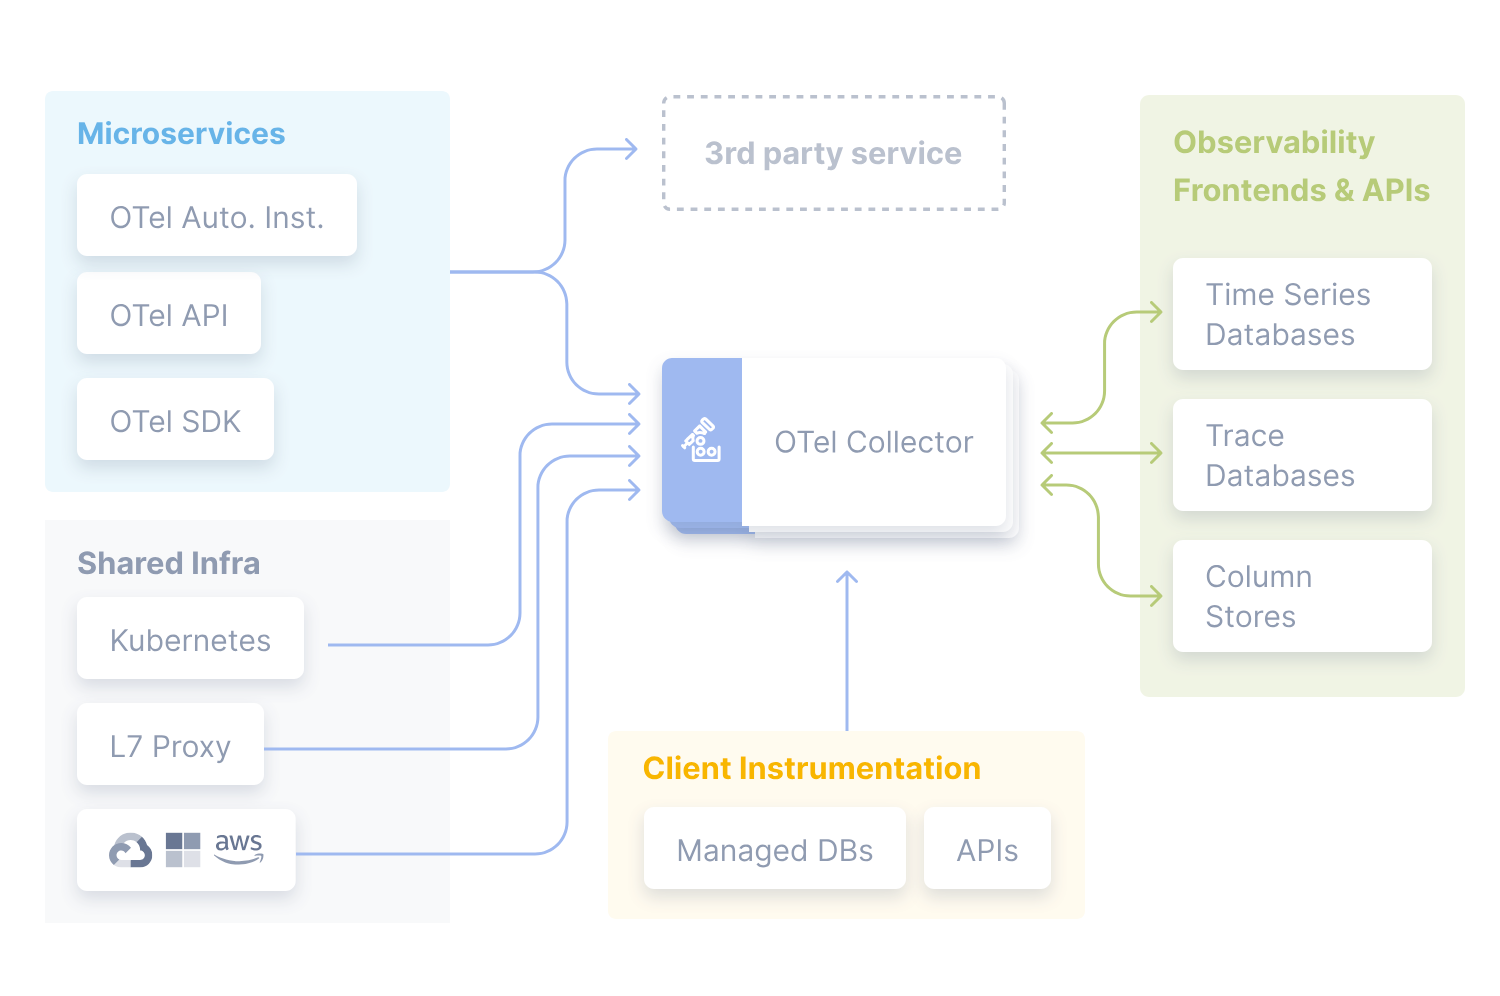
\includegraphics[width=\linewidth]{Images/otelcollector}
					\label{fig:otelcollector}
				\end{figure}
			\end{column}
			\begin{column}{0.25\textwidth}  %%<--- here
				\begin{enumerate}
					\item Instrumentação
					\item Coleta
					\item Envio
				\end{enumerate}
			\end{column}
		\end{columns}
		
		
	\end{frame}
	
	\begin{frame}
		\begin{figure}
			\centering
			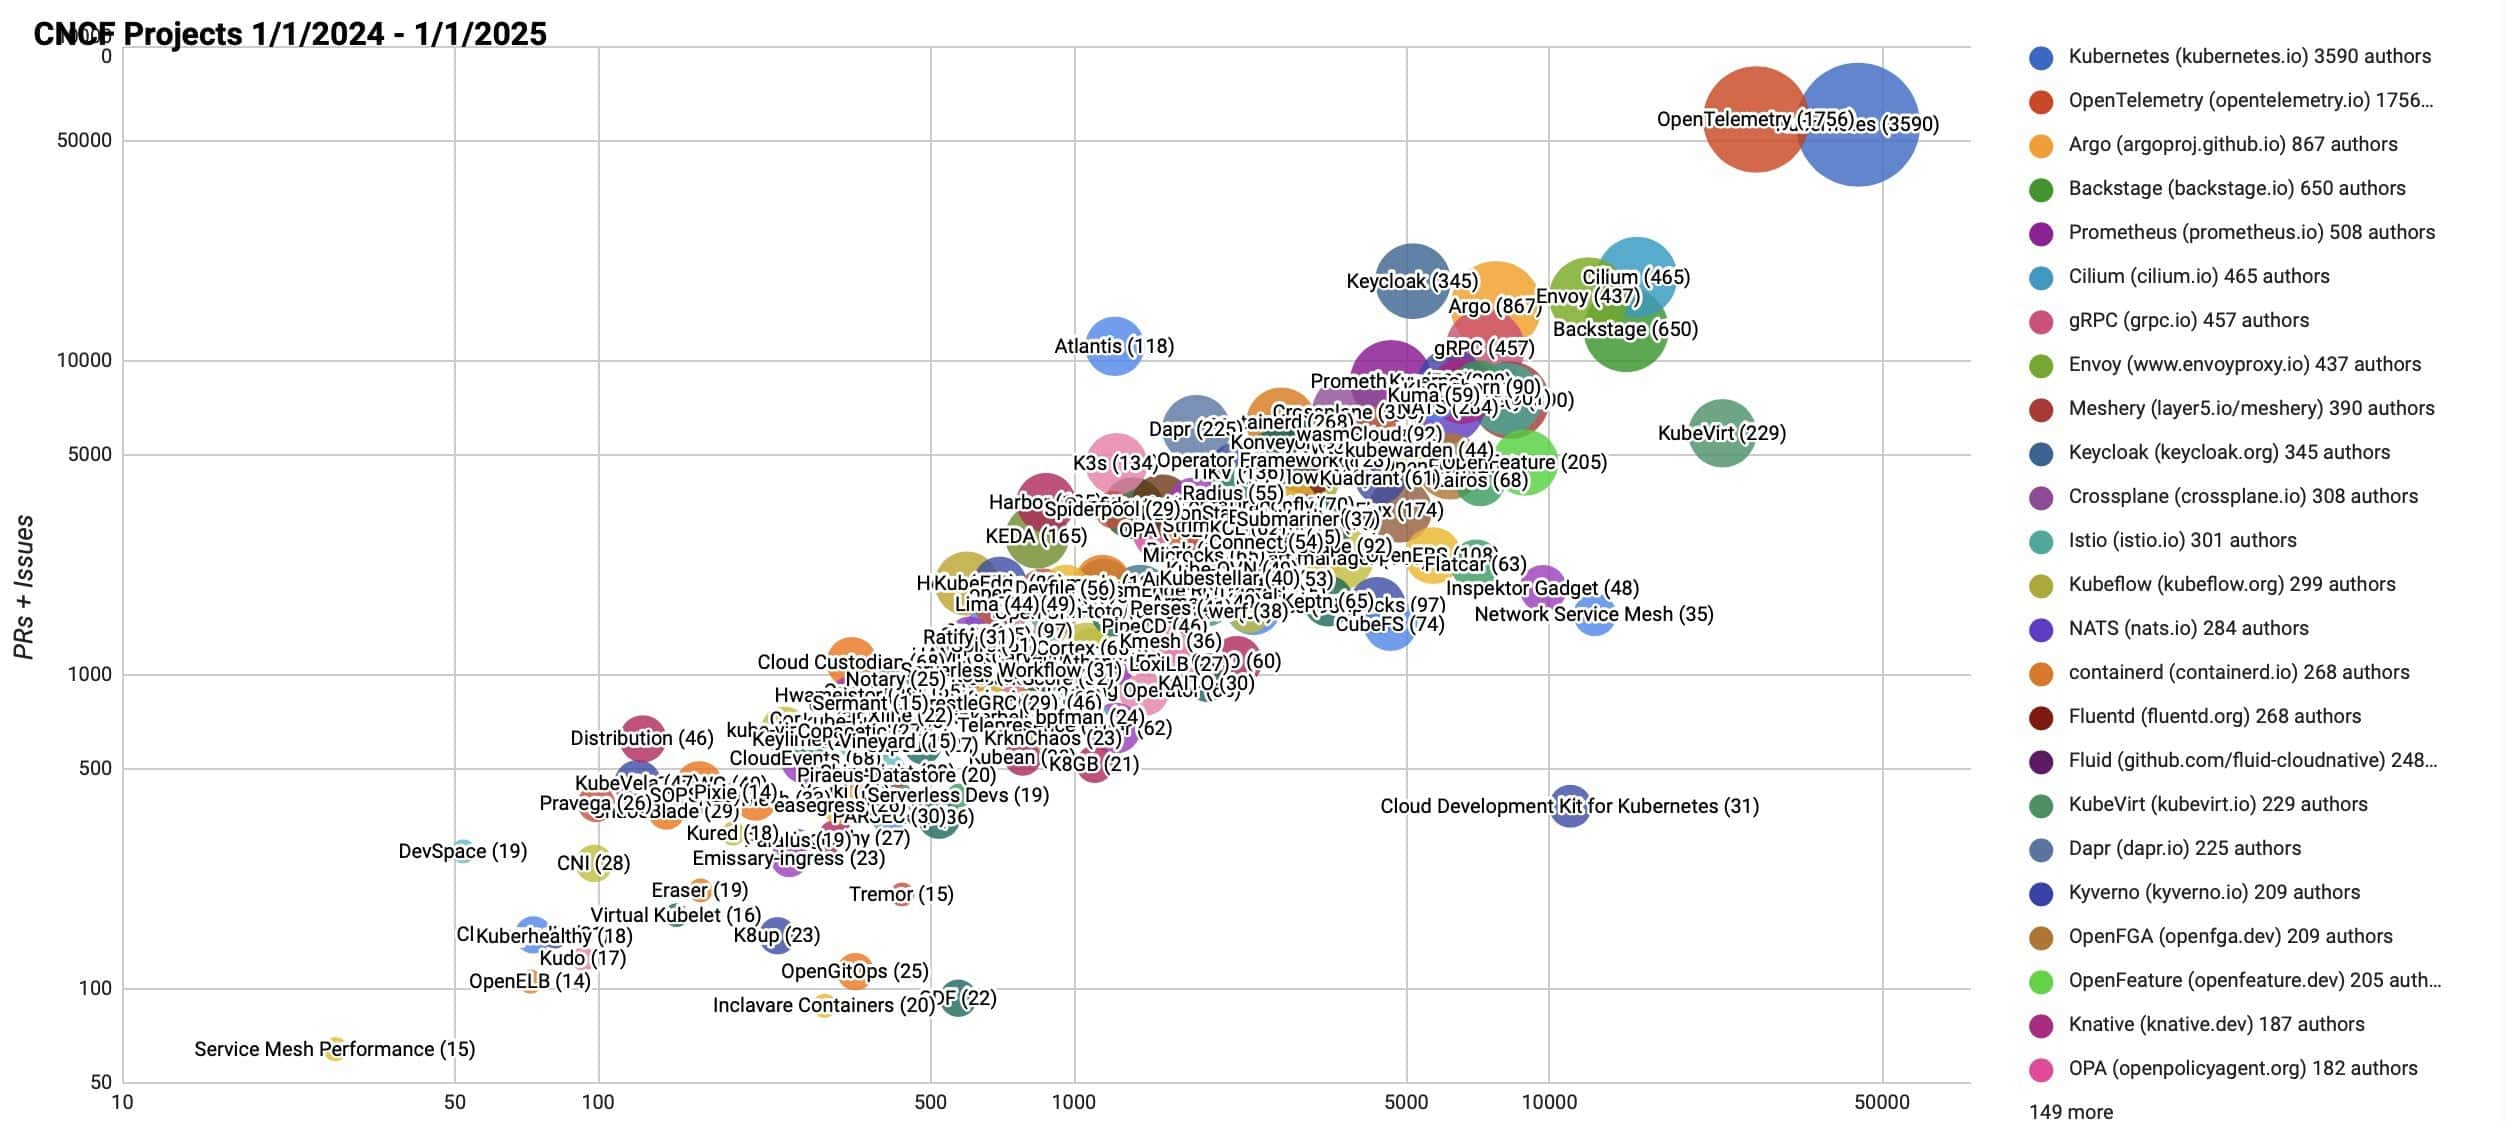
\includegraphics[width=\linewidth]{Images/landscape}
			\label{fig:cncfprojects}
		\end{figure}
	\end{frame}
		
	\begin{frame}{Instrumentação}
		
		\begin{itemize}
			\item {\faCode} \textbf{Biblioteca (Library)}  
			\begin{itemize}
				\item Instrumentação manual usando APIs do OpenTelemetry diretamente no código
			\end{itemize}
			
			\item {\faCogs} \textbf{Framework}  
			\begin{itemize}
				\item Integração com frameworks que já oferecem suporte oficial
				\item Ex: Spring Boot, Quarkus, ASP.NET Core
			\end{itemize}
			
			\item {\faMagic} \textbf{Manipulação de artefato}  
			\begin{itemize}
				\item Instrumentação automática por meio de interceptores, agentes ou manipulação de bytecode
				\item Ex: Java Agent (javaagent), AWS Lambda layer, JavaScript Zero code instrumentation
			\end{itemize}
		\end{itemize}
		
	\end{frame}
	
	
	\begin{frame}{Otel Collector - Upstream}
		
		\begin{figure}
			\centering
			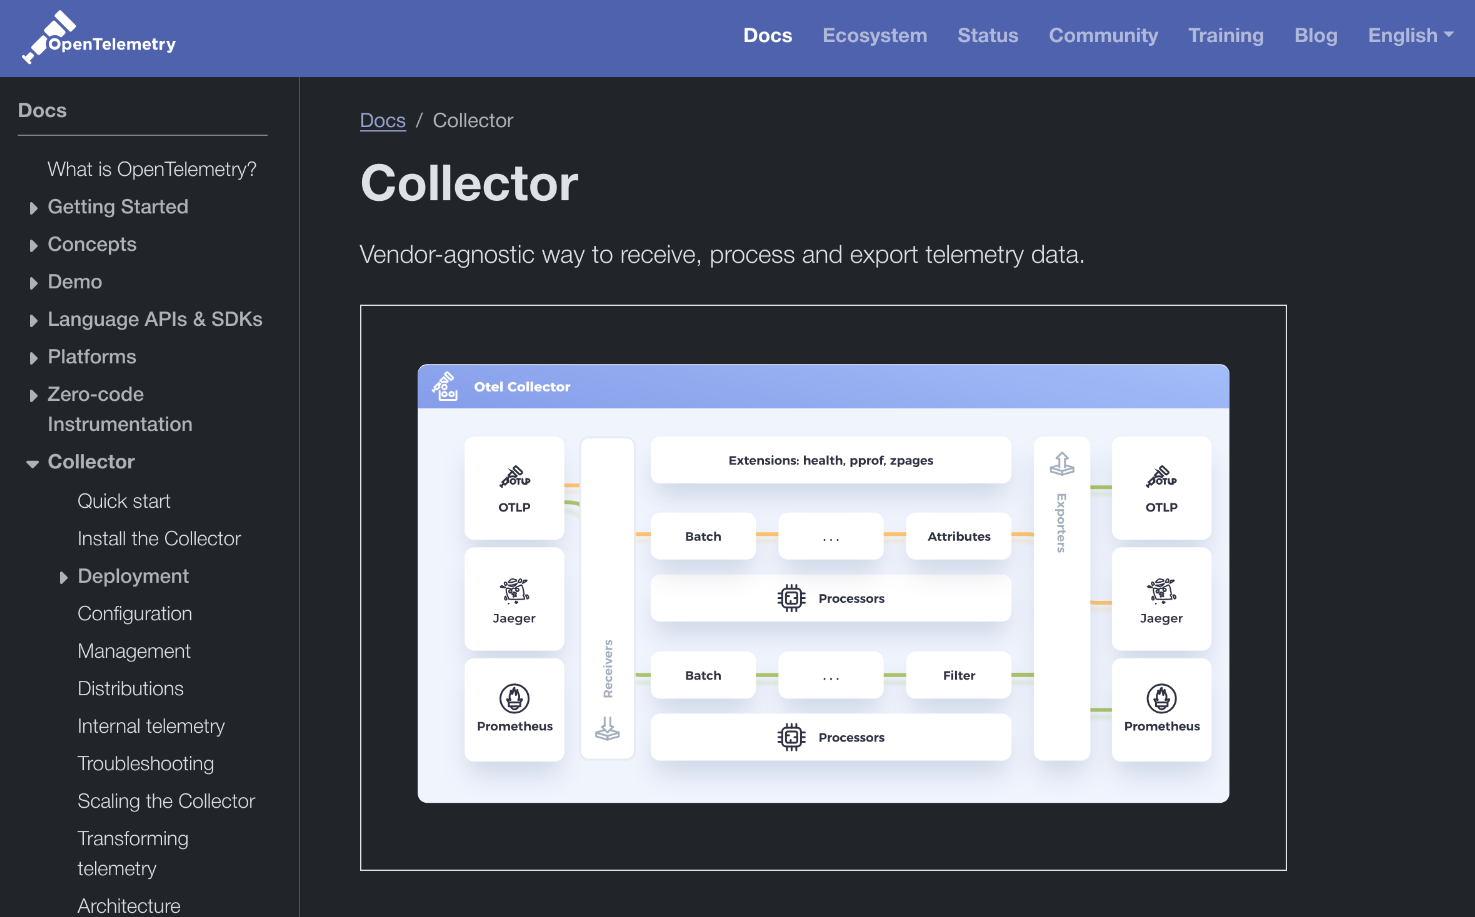
\includegraphics[width=0.7\linewidth]{Images/otelupstream}
			\label{fig:otelupstream}
		\end{figure}
		
		
	\end{frame}
	
	\begin{frame}
		
		\begin{figure}
			\centering
			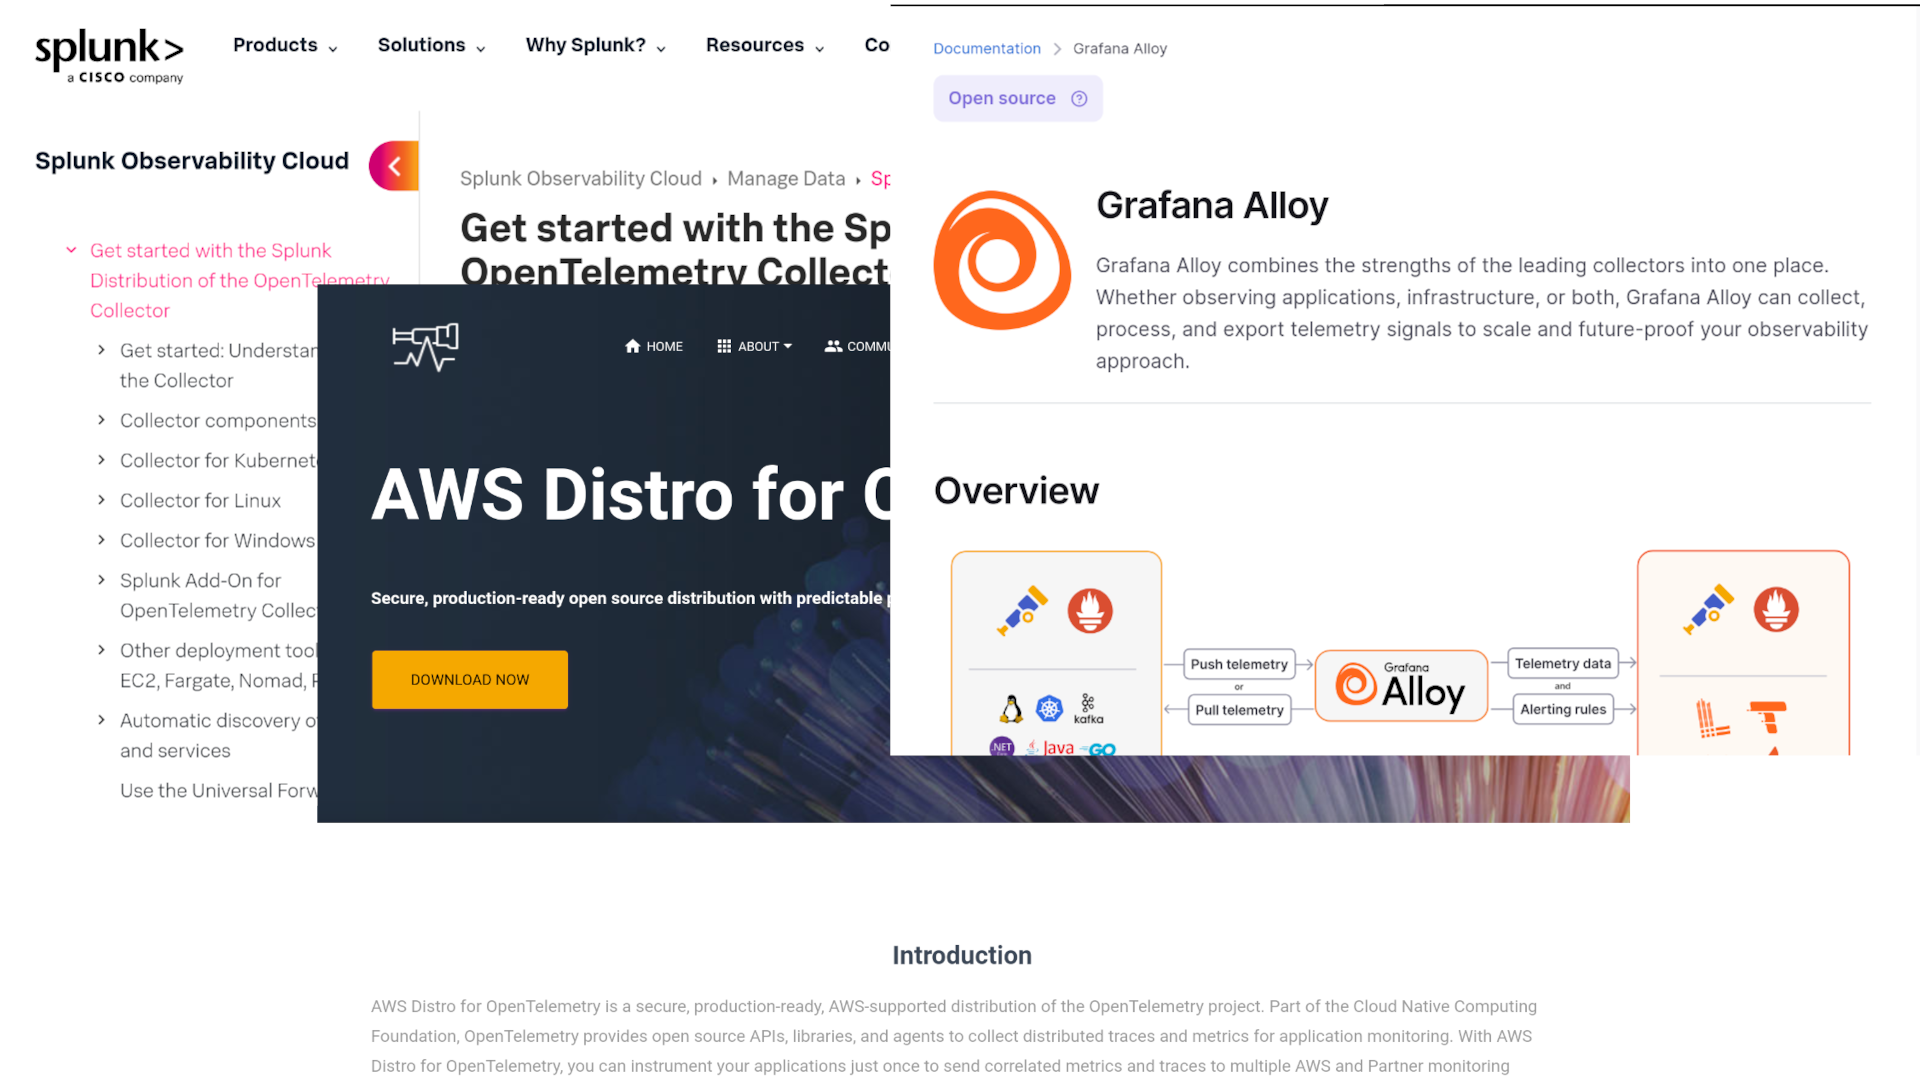
\includegraphics[width=\linewidth]{Images/oteldistros}
			\label{fig:oteldistros}
		\end{figure}
		
		
	\end{frame}
	
	
	
	\begin{frame}
		\begin{figure}
			\centering
			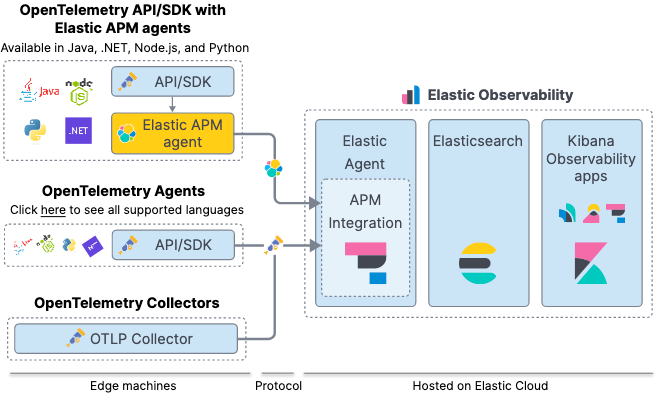
\includegraphics[width=0.8\linewidth]{Images/elasticotel}
			\label{fig:elasticotel}
		\end{figure}
	\end{frame}
	
	\begin{frame}
\begin{figure}
	\centering
	\label{fig:adotcollector}
	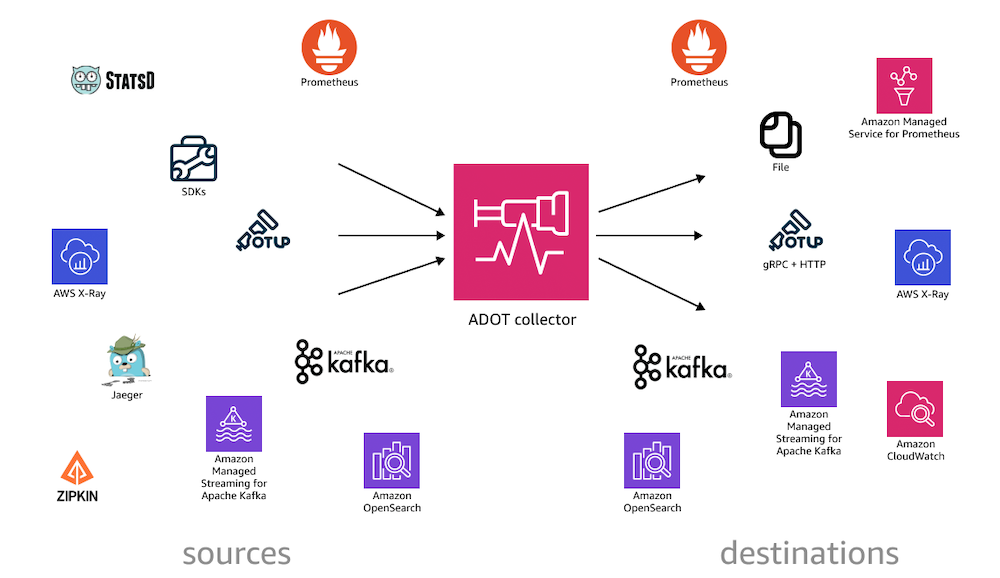
\includegraphics[width=0.8\linewidth]{Images/adotcollector}
\end{figure}
	\end{frame}
	
	
	\begin{frame}{Fatos aleatórios que eu aprendi}
		
		
		\begin{enumerate}
			\item A instrumentação via \textit{agent} é particularmente boa no Java, o problema que ele instrumenta demais
			\item A instrumentação de framework tem um limite quando você pega bibliotecas não -opinionated- ... ela não funciona
			\item A instrumentação via \textit{agent} precisa fine-tunning em cargas de trabalho não permanentes -i.e. faz com que o Lambda fique (ainda mais) lento no boot-
			\item As \textit{distribuições} do collector facilitam o envio de dados
			\item O barco da \textit{padronização} já esta em alto mar, ele chama-se OpenTelemetry
			\end{enumerate}
	\end{frame}
	
	
	{
		\usebackgroundtemplate{
\includegraphics[width=\paperwidth]{Images/separador}}
		\setbeamercolor{normal text}{fg=white}
		\setbeamercolor{frametitle}{fg=red}
		\usebeamercolor[fg]{normal text}
		\section{Exemplo}
	}
	
	\begin{frame}
		
		
		\begin{columns}
			
			\begin{column}{0.5\textwidth}
		\begin{figure}
			\centering
			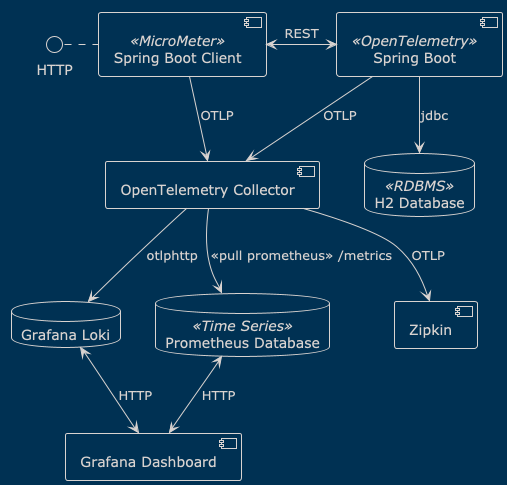
\includegraphics[width=\linewidth]{Images/otel}
			\label{fig:otel}
		\end{figure}		
			\end{column}
			
			\begin{column}{0.5\textwidth}
				\begin{figure}
					\centering
					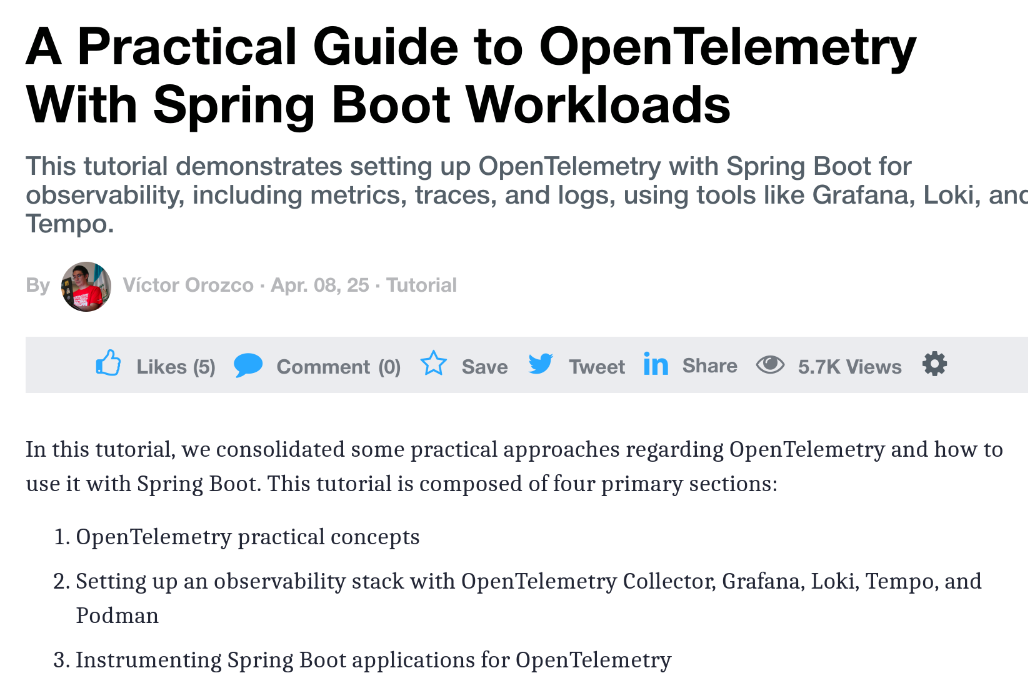
\includegraphics[width=0.7\linewidth]{Images/dzoneotel}
					\label{fig:dzoneotel}
				\end{figure}
\begin{figure}
	\centering
	
\includegraphics[width=0.4\linewidth]{Images/QR.png}
	\label{fig:qrdzone}
\end{figure}
			\end{column}
		\end{columns}
		
		
		
	\end{frame}
	\begin{frame}{Víctor Orozco}
		\begin{columns}[T]
			
			\begin{column}[T]{4cm}
				\begin{figure}
					\centering
					
\includegraphics[width=0.8\linewidth]{Images/logos}
				\end{figure}
			\end{column}
			\begin{column}[T]{6cm}
				\begin{itemize}
					\item vorozco@nabenik.com
					\item \href{https://twitter.com/tuxtor}{@tuxtor}
					\item \href{https://vorozco.com}{https://vorozco.com}
					\item \href{https://tuxtor.shekalug.org}{https://tuxtor.shekalug.org}
				\end{itemize}
				\begin{center}
					
\includegraphics[width=0.1\linewidth]{Images/cclogo}
					\\
					Este trabalho está licenciado sob a licença Creative Commons Atribuição-NãoComercial-CompartilhaIgual 3.0 Guatemala (CC BY-NC-SA 3.0 GT).
				\end{center}
			\end{column}
		\end{columns}
	\end{frame}

	
\end{document}
